
\documentclass[proposal]{umassthesis}  % for Master's thesis
\usepackage{amsmath}

\usepackage{graphicx}
\usepackage{amsfonts}
\usepackage{algorithm}
\usepackage{algpseudocode}
\usepackage{subfig} % This is the package for subfigure environment

\begin{document}

\title{A Machine Learning approach to Precipitation Nowcasting using GPS \protect\\derived Integrated Precipitable
  Water Vapor}

  
\author{Aditya Nagarajan}
\date{May 2016} % The date you'll actually graduate -- must be
                     % February, May, or September
                     
\copyrightyear{2015}
\bachelors{B.E}{Madras Institute of Technology}
\masters{M.Sc.}{University of Massachusetts, Amherst}
\committeechair{David L. Pepyne}
\firstreader{Michael Zink}
\secondreader{Hari Balasubramanian}
\departmentchair{Sundar Krishnamurthy} % Uses "Department Chair" as the title. To
\departmentname{Department of Mechanical and Industrial Engineering}

 \degree{Master of Science}{M.S.}

\frontmatter
\maketitle
%%\copyrightpage     %% not required for an M.S. thesis
\signaturepage

%%
%% Dedication is optional -- but this is how you create it
%%\begin{dedication}              % Dedication page
%%  \begin{center}
%%    \emph{To my loving grandmother Karpagam Krishnamurthy}
%%  \end{center}
%%\end{dedication}

%%
%% Acknowledgements are optional...yeah, right.
\chapter{Acknowledgments}             % Acknowledgements page

%%
%% Abstract is MANDATORY. -- Except for MS theses
\begin{abstract}                % Abstract
It is without question that ground-based weather radar provides an excellent source of information for making real-time assessments and short-term predictions of rainfall - where it is occurring, its intensity, how much has accumulated so far, where it is moving, and so on. Despite their value, weather radars are limited in that, under normal operation, they can only sense active rainfall; they cannot sense the buildup and advection of the atmospheric water in the vapor termed as "precipitable water" which serve as a precursor to severe storms. In this thesis we look at a novel way to predict short term(0-2 hours) precipitation or nowcasting by supplementing weather radar based reflectivity products with GPS derived Integrated Precipitable water vapor products derived from a network of GPS-Met stations. We propose to build a software system to retrieve raw GPS signal data, associated surface meteorological data and radar reflectivity data from publicly available data sources, processing the data to produce spatial-temporal atmospheric water and rainfall information over the Dallas, Fort-Worth Texas region. Using this data the spatial and temporal patterns that atmospheric water exhibits before convective rainfall is analyzed for its potential to predict such events. We then propose an approach involving image processing and image-based machine-learning techniques to develop a tool that takes sequences of gridded atmospheric water fields and gridded weather radar fields and predicts the future gridded rainfall field.
\end{abstract}

\tableofcontents                % Table of contents
\listoftables                   % List of Tables
\listoffigures                  % List of Figures


\mainmatter   %% <-- This line is mandatory


\chapter{Introduction}
Precipitation occurs when the atmosphere becomes over-saturated with moisture, usually caused when warm moist air is uplifted into cooler air. The decrease in temperature reduces the amount of moisture the atmosphere can hold and it precipitates out and falls to the ground. Weather radar can sense where precipitation is occurring, and hence is useful for telling where it is currently raining and with the 5-minute update rate of weather radars such as NEXRAD one can get a sense of where the rain is moving. Weather radar, however, cannot normally sense the atmospheric water vapor or Integrated Precipitable Water (IPW) which is usually evaporated into the atmosphere, since the water molecules are too small to return a sufficient radar return. By measuring changes in refraction of GPS signals as they travel between GPS satellites and GPS ground stations, on the other hand, modern so-called GPS-meteorology techniques can obtain very accurate estimates of atmospheric moisture with update rates of 30 minutes or less. Agencies such as UCAR(http://www.suominet.ucar.edu/) and NOAA (http://www.gpsmet.noaa.gov/) operate a large network of GPS-Met stations and publish point measurements of IPW in near real time. Moreover, with the increasing number of GPS-Met stations over the years, it is possible to combine the IPW measurements of multiple GPS stations to interpolate the IPW or moisture field over the region. While the resulting moisture field does not have the spatial or temporal resolution of the precipitation field produced by weather radar, it can show where the moisture that could later become precipitation is concentrating and where it is moving. In this sense, GPS-meteorology and weather radar would seem complementary to predicting precipitation in that one can sense where the moisture that might become precipitation is concentrating, while the other can sense where the conditions for precipitation have been met. Using the two sources of information, the goal of this proposed work is to develop machine-learning techniques to make short-term(0-3 hours) spatial-temporal precipitation nowcasts to predict the probability of rain at a given spatial location, 1-3 hours in advance of the rain.

The remainder of this proposal is organized as follows. Chapter 2 will overview the atmospheric physics and the principles of the various sensor technologies used to measure the various quantities used in this thesis. This includes an overview of GPS-Meteorology technique and weather radars. Chapter 3 will give a brief literature review pertaining to existing methods of using water vapor information to make forecasts, various machine learning applications in meteorology and the state of the art machine learning algorithms used for supervised and unsupervised learning by exploiting the spatiotemporal information in a sequence of frames or video inputs. Chapter 4 will introduce the preprocessing steps to derive IPW and the interpolation technique to generate the moisture fields. Using these fields along with reflectivity fields we present initial results of precipitation forecasts. Chapter 5 will discuss the proposed contributions that this thesis will make, our existing contributions and the plan moving forward. 


%Chapter 3 will describe techniques for interpolating point GPS-meteorology measurements of water vapor to obtain estimates of moisture fields. Chapter 4 will then give a literature review of some current approaches for precipitation forecasting using GPS-meteorology derived moisture measurements as well as some related weather radar-based precipitation forecasting techniques. Chapter 4 will also review some of the video, image processing, and machine-learning techniques that are motivating the development of our machine-learning technique. Chapter 5 gives some preliminary results, describing our method for GPS and weather radar data processing, the current machine learning technique that we are exploring, and some early learning results. The document closes with Chapter 6, which gives our plan and timeline for completing our proposed work as well as a listing of the expected contributions we hope our work will make.

\chapter{Background}

To get an insight on making predictions of rainfall and amounts of rainfall we first look at the fundamental atmospheric physics that drive the precipitation processes. We do a brief survey in the domain of meteorology to see what factors drive the rainfall processes and other severe storms. 

The fundamental approach that we have taken in this work relies heavily on remotely sensed meteorological parameters such as water vapor from GPS-Meteorology technique and rainfall intensities from NEXRAD dual polarized weather radars. This chapter will explain the principles behind these two remote sensing systems. We will also describe the methods and sources used to build our data set.

GPS-Meteorology sensors measure the amount of atmospheric water vapor through signal delays that are incurred due to atmospheric refraction. The fundamental measurement that is thus obtained is refractivity and this refractivity is mapped to the amount of Integrated Precipitable Water Vapor(IPW). 

IPW can be defined as the depth of water in a bucket with 1 square meter opening measured in mm that you would get if all the water vapor measured above sensor were to suddenly precipitate out as liquid.

Weather radars use microwave signals to detect precipitation in the form of rain, hail and snow once they have developed large enough to return radar echoes. The signal strength of those singles that are returned are mapped to the rainfall intensity measured in dBZ. The fundamental measure in this case is reflectivity. 

\section{Precipitation Basics}

Water vapor is one of the most fundamental quantities in the atmosphere which is responsible for various weather events such as thunder storms, hurricanes heavy rainfall and flash flooding. The release of latent heat when water vapor changes from one state to another is associated with the formation of severe thunder storms. 

The hydrological cycle shown in Figure \ref{fig:weather_cycle} is a series of processes where water is transformed from one state to another. To understand the processes of rainfall we need to know the amount of water vapor also termed as "precipitable water". Water vapor is usually measured in relative terms known as relative humidity, which is a measure in terms of  percentage. A measure of relative humidity gives us the measure of saturation of the water vapor. This means that when we have 100 \% relative humidity the air can not hold any more water vapor and thus it has to compensate by some of it condensing out into clouds. It is not necessary that water vapor reach a relative humidity level of 100 \% in order for it to start condensing into clouds. Temperature to a large extent plays a role in the amount of water vapor the atmosphere can hold. At higher temperatures air can hold much more water than at lower temperatures. The temperature at which water vapor starts forming into clouds is called the dew point temperature. Thus there exists a particular temperature where the air is saturated and can not hold any more water vapor and at this point, water vapor starts condensing out into clouds. 

The cooling of air can happen in many ways such as vertical uplifts of cold air or horizontal movement of cold air such as sea breeze. When a parcel of air rises it tends to expand and this expansion results in a decrease in temperature, thus this decrease in temperature will cause water vapor to condense into what is generally termed as clouds. We derive a term called lapse rate from this processes defined as the decrease in temperature in celsius per kilometer of rise in air. Clouds are generally formed from air being lifted. 

In order to predict the the weather it is useful to know the vertical temperature and relative humidity profile. Vertical and horizontal distributions of water vapor are very useful quantities in predicting the weather. Relative humidity is usually measured as a surface based quantity which are measured by a network of in-situ weather stations. A more useful quantity is the vertical distribution of water vapor which is obtained from radiosondes and satellite imagery. A variety of remote sensing based water vapor detection techniques include water vapor radiometers, LIDER, and GPS-Meteorology exist. The water vapor measurements used in this work are primarily from the GPS-Metrology technique which is detailed in the next section. 
\begin{figure}[t]
\begin{center}
\label{fig:weather_cycle}
\includegraphics[width = 0.6\textwidth]{weather_cycle}[!h]
\caption{Observations from satellite i,j received at receiver l,k (figure taken from \cite{ming2014})}
\end{center}
\end{figure}

Radiosondes are a set of instruments which are launched up to 30km into the air that measure atmospheric parameters while it descends down on a balloon. Typically radiosondes are launched 2 times a day at the same time world wide at 0000UTC and 1200UTC. The cost of launching radiosondes limits the spatial resolution of water vapor. 

Ground based water vapor radiometers measure the background microwave radiation emitted by atmospheric water vapor along a given line of site. This method has several drawbacks in that the instrument has to be carefully calibrated, they are too expensive and they do not work during heavy rainfall.  

GPS-Meteorology thus provides us with a low cost method of measuring water vapor, and by constructing a network of GPS-Met stations we are able to get a very precise spatial and temporal sampling of water vapor. 
%Our atmosphere consists of a wide range of dynamic processes which drive severe weather events and precipitation. Precipitation occurs as a result of water vapor condensing into clouds which after reaching its saturation point turns into precipitation. This saturation extent is related to the temperature. Water vapor is also the cause of severe thunder storms and convective weather due to the release of latent heat when it changes its phase. The dew-point is defined as the temperature at which net-condensation of water is higher than net-evaporation. 
%
%The basic principle behind cloud formation lies decreasing temperatures which reach the dew-point temperature and form clouds. A common way that for condensation to occur is warm air rises and expands and thus cools the surrounding atmosphere which in-turn brings the temperature to the dew point temperature thus forming clouds. 

% For weather prediction applications it is essential to know the distribution of water in the "gas" phase which is termed as water vapor or "precipitable" water. It is also vary difficult to measure water in this phase that is most important to us. Some of the existing techniques to measure water vapor are radiosondes or weather balloons which measure atmospheric parameters as the balloon descends to earth, raw insondes which use microwaves to determine water vapor content and GPS-Meteorology which use signal propagation delays to estimate the amount of water vapor. 
%
%A measure of water vapor may sometimes be measured as relative humidity. Relative humidity is measured in percent where 0\% means there is no water vapor in the atmosphere and 100 \% indicates the atmosphere is saturated and can not hold any more water vapor, and additional water vapor evaporated in the atmosphere will have to be compensated by it being condensed into tiny ice crystals which together form into clouds. The saturation point also depends on the temperature, thus at higher temperatures the atmosphere can hold more water vapor. The rate of condensation is generally associated with vapor pressure and does not depend on temperature. The dew-point is defined as the temperature at which net-condensation of water occurs rather than net-evaporation. It can also be stated as the temperature at which a unit air must be cooled in order for the water vapor to saturate. 
%
%There are two different types of clouds stratiform clouds which stay in one place and produce light drizzles and convective clouds that are in constant motion and produce heavy rain as they move. 
%
%cumulonimbus : clouds which cause severe thunder storms due to vertical convective air. 
%stratiform clouds are much thinner layered clouds which produce rainfall of lesser intensities but last a long time. 

%This chapter gives a background to describe how weather radar and the GPS-meteorology technique work and what each of the two sensors can detect and measure. This chapter also describes some of the basic interpolation techniques that are used to map point measurements of GPS-meteorology derived water vapor to 2- and 3-dimensional moisture fields.

\section{GPS Meteorology Technique}
\subsection{GPS Overview}
GPS is a system of satellites operated by the Department of Defense(DoD) in the United States first launched 1980s for the purpose of military navigation. The GPS system was later introduced for civilian purposes. The GPS satellites is a constellation of 24 different satellites flying at 22,200 ft AGL operational at any given time orbiting in 6 different orbital planes inclined at $55^{\circ}$ to each other \\ (http://www.gps.gov/systems/gps/space/). At any given time it takes 4 satellites to determine a particular location on earth. To determine the position a technique called triangulation is used where the distance from each satellite is measured and the (x,y,z) coordinates is determined by solving the system of equations or finding the intersection of the three spears which is the position. The 4th satellite is usually used to compensate for the clock errors between the position on earth and the satellites. 

GPS satellites transmit carrier signals in two distinct frequency bands $L_1$ band ($f_1 = 1575.42 MHz$) and $L_2$ band ($f_2 = 1227.60 MHz$) which are reserved for GNSS applications alone. These signals are modulated as a sequence of bits called Pseudo Random Noise(PRN) and each satellite has a unique PRN code which changes periodically \cite{hoffman2008gnss}. A receiver on the ground capable of operating in these two frequencies measures two fundamental quantities from the GPS signals, the pseudo range which measures the distance the signal has travelled from the satellite to the receiver in meters and the carrier phase which is the number of wavelengths travelled by the signals measured in number of cycles. Using carrier phase measurements in calculating position is more accurate than using pseudo ranges(looking for citation). 
\subsection{Analysis of GPS signal delays}

As GPS signals propagate from the GPS satellite to the receiver they are retarded by many different factors. This retardation causes an error in the calculation of the position of a body on the ground. The error in calculation is mainly because of the excesses path distance the signal has travelled than it ideally should have. Some of these errors include receiver and satellite clock bias, ionospheric delay, tropospheric delay and other residual errors such as multi path and improper modeling of antenna phase center variations. This excesses path distance can be summarized with the following expression expressed in number of cycles, 
\begin{figure}[!t]
\begin{center}
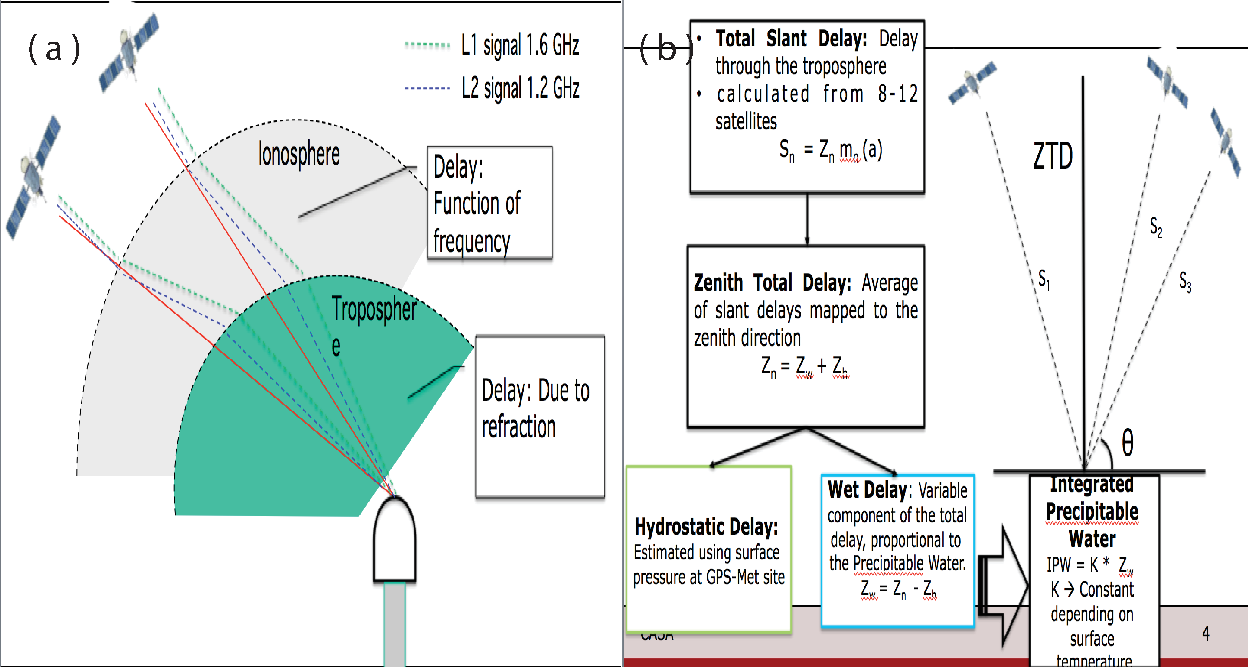
\includegraphics[width = 0.9\textwidth]{GPS_Met_Basics}
\caption{Signal path delays from (a) satellite to receiver, (b) Tropospheric delays}\label{fig:GPS_Met_Basics}
\end{center}
\end{figure}
\begin{equation}
L_r^s  = G_r^s - (\delta t_r - \delta t_s) * c +  \lambda \cdot N_r^s + \delta_{r,ion}^s + \delta_{r,trop}^s + \xi
\label{eqn:totDel}
\end{equation}
where $L_r^s$ is the phase difference between the reference and the receiver carrier, $G_r^s$ is the geometric path distance between satellite $s$ and receiver $r$, $\delta t_r, \delta t_s$ are the clock biases between the receiver and satellite clock respectively,  $c$  is the speed of light, $\lambda$ is the wavelength of either the $L_1$ or the $L_2$ signal, $\delta_{r,ion}^s$,  $\delta_{r,trop}^s$ are the ionospheric and tropospheric delays respectively and $\xi$ is the remaining residual errors such as multi path etc. Figure \ref{fig:GPS_Met_Basics}a gives a basic schematic of the signals traveling in space from satellite to the receiver. These delays need to be accounted for use in highly accurate geodetic positioning and tectonic shift monitoring used by geodesists and geophysicists \cite{leick2015gps} \cite{abdrakhmatov1996relatively}. While these are considered errors in this field, the ionospheric and tropospheric delays can be used to study the respective media. Particularly the tropospheric delays are of great use to meteorologists as variability in time due to this delay is proportional to the variability in the water vapor content in the troposphere  \cite{bevis1992gps} \cite{rocken1995gps} \cite{duan1996gps}. This technique has also been validated to produce water vapor measurements of better than RMS 2mm \cite{duan1996gps}. The remainder of this thesis focuses on using this delay component mapped to the amount of precipitable water. The following two sections provide the reader with a brief overview of modeling and removing the GPS signal delays in Equation \ref{eqn:totDel}.

\subsubsection{Modeling the Ionospheric delay}
The delay in the ionosphere is mainly caused by dispersion. The two operating frequency ($L_1 \  and \ L_2$) are affected differently by this dispersion \cite{spilker1980gps}. 99.9\% of the ionospheric delay can be accounted for by the first order ionospheric combinations given in \cite{herring2015gamit}. 

\begin{equation}
I_1 =  \dfrac{-40.3 \int\ N_e dl}{f^2}
\end{equation}

Where $N_e$ is the electron content along the path. This error is accounted for by using dual frequency measurements applied to a well known technique called ionospheric free linear combination given in\cite{blewitt1990automatic}. 
\begin{equation}
L_3 = \dfrac{1}{f_1^2 - f_2^2} * (f_1^2L_1 - f_2^2L_2)
\label{eqn:ionFree}
\end{equation}

Thus the $L_3$ signal contains the signal with all other delay components other than the ionospheric delays. 

\subsubsection{Modeling satellite and receiver clock errors}
\begin{figure}[t]
\begin{center}
\includegraphics[width = 0.5\textwidth]{gps_doubl_differences}
\caption{Observations from satellite i,j received at receiver l,k (figure taken from \cite{ming2014})}\label{fig:dd_satellites_receivers}
\end{center}
\end{figure}
The technique of double differencing relies on the assumption that by subtracting the ionospheric free linear combination observed at two different stations, the common errors between the signals will be mitigated which leaves us with errors due to satellite orbit, multi path errors, tropospheric error and errors due to phase center variations \cite{alber2000obtaining}. The single difference is combining observations from a single satellite observed at two different stations. From Figure \ref{fig:dd_satellites_receivers} would be combining the linear combinations from satellite i observed at receiver l and receiver k given by the equation 
\begin{equation}
s_i^{lk} = L_k^i - L_l^i  \quad \textrm{and} \quad  s_j^{lk} = L_k^j - L_l^j
\label{eqn:singlediff}
\end{equation}

where the L in this equation refers to the ionospheric free linear combination obtained from \ref{eqn:ionFree}. The double difference equation is then expressed as the difference between two single difference equations given by
\begin{equation}
dd_{ij}^{lk} = (L_k^i - L_l^i) - (L_k^j - L_l^j) = s_i^{lk} - s_j^{lk}
\end{equation}

This however does not address the issue of site correlations. In order to address the site correlation baseline(distances between two sites) must be greater than 500km. This would mean that two different stations see the same satellite at completely two different elevation angles(citation needed). A key drawback of this technique is that the slant path delay along the ray path are lost due to the double differencing \cite{ware1997sensing} and to obtain these delays one needs to estimate the zenith delays first. 

\subsubsection{Modeling Tropospheric delays}
 95.0\% of the atmospheric water vapor resides in this region and hence our focus will be on extracting the tropospheric delay. Delay due to water vapor in the troposphere is mainly due to the refraction and this delay is proportional to the refractivity. The Slant Total Delay(STD) in the troposphere is given by \cite{bevis1992gps}
 \begin{equation}
 STD = 10^{-6} \int\limits_S N ds - G
 \end{equation}
where S is the signal path and G is the geometric distance between the satellite and the receiver and N is the refractivity of the troposphere. The closed form expression for refractivity is given by the following expression. 
\begin{equation}
N = 77.6 (\dfrac{P_d}{T})  + 64.8 (\dfrac{P_w}{T}) + 3.776 \cdot 10^{5} (\dfrac{P_w}{T^2})
\end{equation}

where $P_d$ is the partial pressure of dry air and $P_w$ is the partial pressure of water vapor. 

In our analysis however delays are estimated using the GPS signal propagation delays. The delay in the troposphere can be broken down into two main components, hydrostatic(dry) delay and the wet delay \cite{saastamoinen1972atmospheric} \cite{davis1985geodesy}. The delays are typically averaged from each satellite in view(8-12) and mapped onto the zenith component termed as the Zenith Tropospheric Delay(ZTD). Thus the Total slant delay seen at an elevation angle $\theta$ from the GPS antenna is given by
\begin{equation}
S_{\theta} = ZTD \cdot m(\theta)
\end{equation}
where $m(\theta)$ is termed as the mapping function is approximately 
\begin{equation}
m(\theta) = csc(\theta)
\end{equation}
Separating out the Zenith Total Delay into the hydrostatic part and the wet part 
\begin{equation}
S_{\theta} = ZWD m_w(\theta) + ZHD m_h(\theta)
\end{equation}
where ZHD and ZWD are the zenith components of the hydrostatic and the wet delays respectively and $m_h$ and $m_w$ are the hydrostatic and wet mapping functions respectively. At elevation angles $15^\circ$ we can lump the wet and the dry mapping function onto a single mapping function 
\begin{equation}
S_{\theta} = ZTD m_n(\theta)
\end{equation}
and $m_n$ is defined as the neutral mapping function and ZTD is 
\begin{equation}
ZTD = ZHD + ZWD
\end{equation}
The water vapor dependent component of our interest is the ZWD which can be extracted by estimating ZHD given in \cite{saastamoinen1972atmospheric}
\begin{equation}
ZHD = \dfrac{0.00227768 P_0}{1 - 0.00266 cos(2\phi) - 0.00028h_{ref}}
\end{equation}
where $P_0$ is the surface pressure at the site, $\phi$ is the site latitude and $h_{ref}$ is the height of the station. 
We can obtain the ZWD by subtracting the ZHD from ZTD and map it to the amount of IPW given by \cite{bevis1994gps}
\begin{equation}
IPW = \Pi ZWD
\end{equation}
where $\Pi$ is a function of surface temperature and the ideal gas law constant.  A summary of the tropospheric delay modeling is given in Figure \ref{fig:GPS_Met_Basics} b. The implementation of the above processes is done using the GAMIT software and estimation of IPW at each station is obtained given the pseudo range/carrier phase observations at the stations and the meterological parameters at the stations. 

\subsection{GAMIT GPS analysis at MIT}
GAMIT is a software package developed at MIT \cite{herring2015gamit} used for high precision GPS analysis. It uses the double differencing technique and the tropospheric delay models to determine the IPW at a given station. The ZTD(Zenith Tropospheric Delays)  are modeled as a first order Gauss-Markov processes \cite{tralli1990stochastic}. This is based on the assumption that the signal delays remain constant over a small period of time. 

The input to the GAMIT software packages are the RINEX(Receiver Independent Exchange Format) observation, navigation and meteorological files \cite{gurtner2007rinex} which are a set of file formating protocols  universally defined for logging data from GNSS receivers from multiple manifacturers. The satellite orbital parameters for each satellite which are generated by the IGS(International GNSS services) \cite{dow2009international} are also an input to the processes which are automatically downloaded by GAMIT for the time period of the analysis. The RINEX observation files contain the carrier phase and the pseudo range measurements sampled at 30s intervals, the RINEX navigation files contain the receiver satellite clock offsets and the RINEX meteorological files contain the pressure temperature and relative humidity at each station. Reference stations with baseline of over 500 km are chosen to determine the absolute value of IPW at each station. 

\section{Principles of Radar Meteorology}

The primary sensor to detect severe weather and and precipitation are the Next Generation Weather Radars (NEXRAD) or WSR-88D which stands for Weather Surveillance Radars 1988 Doppler radars. The National Weather Services and a consortium of agencies including the FAA, US DoT, DOD operate a total of 160 radars in the United states. The information obtained from these radars are precipitation rate and wind velocities. 

The WSR-88D are a dual polarized doppler based radars operating in the S-Band(2-4 GHz). The dual refers to the horizontal and vertical polarization which enables the radar to better detect the what the signal is reflecting. This includes clearly distinguishing between rain, hail, snow, ground clutter and birds. The basic principle of the radar is that it releases a pulse into space and measures the magnitude of the reflected pulse which is directly proportional to the intensity of the the reflected object(rain, hail, snow). This signal is them processed to be displayed on a mosaic map to reflect the location and intensity of the precipitation. This intensity is measured in dBZ. 

The NEXRAD radars are preprogrammed to nine different VCP (Volume Coverage Scans) which can be controlled by the NWS meteorologists based on specific weather events. 
\chapter{Literature Review}

This chapter gives a literature review relevant to our goal of using spatial-temporal GPS-meteorology derived moisture and weather radar sensed precipitation to make short-term precipitation forecasts (nowcasts).

As such the chapter will review other attempts to use GPS-meteorology for precipitation forecasting as well as other attempts/approaches for using weather radar data for precipitation forecasting. In doing the review, we will touch only very lightly on the model-based approaches to forecasting such as numerical weather prediction, since approach is machine learning based and not model based.

As background for our spatial-temporal machine learning techniques, this chapter will review relevant and motivating work from the areas of video processing, image processing, and machine-learning.

A great deal of effort has been made to make GPS derived IPW in real time \cite{ware2000suominet} \cite{wolfe2000developing}. 
\section{IPW from GPS-Met technique used in Forecasting}
Water vapor plays an important role in the atmosphere as a precursor to severe storms and convective rainfall. This is mainly due to the latent heat which is released when water vapor changes phase, from the vapor phase to the gasious phase in the form of clouds or from the vapor phase to the liquid phase in the form of rain. Until the advancements made in GPS-Meterology to accurately measure water vapor \cite{bevis1992gps} \cite{duan1996gps} using GPS signal delays, we are able to get a much better understanding of its role in storm formations. With efforts to make near real time water vapor data available \cite{wolfe2000developing} to weather forecasters, we can use this information to detect storms in advance. 

A key requirement of studying water vapor evolution is dense sampling in space and time of water vapor. To achieve this a network of GPS-Met stations are required. Japan thus far has the most densely operating network of GPS-Met stations with an average station spacing of approximately 17km(looking for citation). It is there fore natural that many studies on the impact of water vapor on short term weather forecasting have been conducted. One such study by \cite{inoue2007characteristics} was conducted to study the predictive potential of water vapor over the Kanto district during the summer months of 2001-2005. Convective storms predictions were done by analyzing the distinct variation in the diurnal cycle of water vapor. Observations of distinct diurnal variation of water vapor were made during during active thunder storm dates. A connection between the lightnings detected using CG (Cloud to ground strokes) using VHF an LF sensors as an index of thunder storm activity. As an indication of convective activity one hourly accumulated rainfall of radar AMeDAS were used. A relation between convective events and PWV were invistigated in each grid in the Kanto district. Large PWV variation would relate to the occurrence and development of convective storms. It was observed that the time variation of IPW precedes that of CG strokes by 1~2 hours. The time with maximum IPW was also 1~2 hours behind maximum R/A. The key observation was a large variation in IPW was correlated with days with severe convective weather. An analysis with maximum occurance of CG strokes and the gradient or variation of water vapor was conducted and belived to be around 1 to 2 hours. The paper concludes by stating that for the limited cases analyzed GPS derived IPW reflect well with local variations in thunder storms. We used R/A and CG stroke for the index of convective activity of thunderstorms. whereas the maximum PWV generally preceded the maximum R/A and CG stroke by 1~2 hours.

An another study \cite{radhakrishna2015precipitable} suggests the variations of horizontal spatial distribution of water vapor are associated with convective events 1~3 hours prior to the event. An interpolation technique similar to the one used in this paper called the Kringing technique \cite{tabios1985comparative} was used to generate IPW fields over the contiguous United States. The information from the humidity maps were studied with regard to meso-$\beta$ scale events(20-200km) and convective initiation. This paper evaluates deviation of moisture fields from the mean for a particular hour in determining large moisture build up 3 hours prior to convective initiation. The events for convective initiation are found using radar reflectivity mosaics and a convective event was defined as anything above 40 dBZ. 

\section{Nowcasting Approaches}

A current Nowcasting approach used by emergency managers for decision support uses high resolution CASA X-band radar network coupled with the DARTS(Dynamic and Adaptive Radar Tracking of Storms) algorithm \cite{ruzanski2011casa}. The DARTS algorithm tries to predict the radar reflectivity fields 15-18 minutes in advance in order to determine the scan pattern of the CASA network of radars. The algorithm analyzes the reflectivity fields in the Fourier Domain along with the velocity fields in the x-y direction. The DARTS algorithm is based on the area based reflectivity nowcasting algorithm. This is an extrapolation method which heavily relies on radar data and uses an advection model to extrapolate current radar reflectivity in space and time.

One of the first applications of machine learning applied to nowcasting was \cite{french1992rainfall}. A nowcasting technique was developed where the model was trained on the current time step of a rainfall field with the rainfall field 1 hour push forward in time. The fields were trained using a single hidden layer artificial neural network using a single frame of  simulated rainfall field from a $100 \times 100$ domain with a resolution of 4km, and thus had 625 grid points as input and the output was the field 1 hour forward in time with the same resolution. The fields that were generated were from a simulation model and the authors had plenty of data to play around with. A simulated field was used because the results did not depend on the data quality. A mathematical model was used to generate the true rainfall field. The performance of the Neural Network was measured against two quantities, the MAI (Mean Areal Index) defined as the mean intensity of the 625 points and the PAC (Percent Areal Coverage). The Neural network model was compared against other nowcasting and persistence approaches and concluded that the Neural Network performed at comparable levels as the latter two. 

Recent developments have been made in applying machine learning techniques to predict convective initiation using GOES(Geostationary Operational Environmental Satellite) satellite imagery data \cite{mecikalski2015probabilistic}. The technique was used to predict a convective storm 0-60 minutes in advance using GOES-R satellite data and NWP data to give probabilistic estimate of CI event or no event using trained separately on two different classifiers logistic regression and random forest. The feature importance metric of the random forest was used to determine the most contributing factors from GOES and NWP data to make the probabilistic predictions. The accuracy of predicting a Convective Initiation event was 84 \% and 71 \% for logistic refression and random forest respectively. 

\section{Recent development in Machine Learning}
A challenge faced in our problem is that we want to use frames of advecting moisture fields and advecting reflectivity fields and thus we have 2 video inputs(frames of moisture and reflectivity images) make accurate precipitation nowcasts. We explore a field of study in machine learning called multi view learning \cite{sun2013survey}. Multi view learning is an unsupervised learning method used find features given two sets of highly correlated features, ex. audio and video input to a classifier to learn a task. 

In particular we were motivated in how people deal with two sets of correlated features. Such a technique was used to learn human emotions with facial expressions and body gestures as input \cite{shan2007beyond}. They extract spatio-temporal features from video input as their primary feature set using a seperable linear filter. A reduced representation of the video sequence was extracted using a series of filters which only captures motion. The study relys on the assumption that the integration of facial expressions and gestures occur very early on in human processing stream. Thus they use the CCA(Canonical Correlation Analysis) method to find a joint-space representation of facial expressions and gestures. The CCA is used to fuse both these features. The CCA method works by finding a set of representations in a space which maximizes the correlation between two different multidimensional vectors. This new feature space is used with a SVM using a Radial Basis Function kernel to classify the different emotions. A comparison of the classification accuracy was made between concatenating the two feature vectors and by using the CCA technique which performed much better. 

A similar application of CCA is found in regressing financial time series data \cite{guo2014feature} where stock market prices was predicted using a set of features that was fused using the CCA technique. The two features were economic factors and and historical data or technical variables. These two features being correlated and complementary were fused together using the CCA technique to predict the closing price for the stock market the next day using a Support Vector Machine Regressor with a Radial Basis Function Kernel. 


\chapter{Methods and Initial Results}
This chapter will describe our data processing approach, machine learning algorithms and methods to evaluate and the performance it gives us. 

The region of interest that was chosen for this study was the Dallas Fort-Worth area. CASA ERC (Collaborative Adaptive Sensing of the Atmosphere Engineering Research Center) has wide ranging interests in this area which includes a test bed consisting of a network of short range dual-poalimetric weather radars as well as other sensors. The center has also established a good relationship with the local NWS (National Weather Services) weather forecasters, emergency officers and public officers. This region is also prone to very volatile weather in the form of severe tornadoes and other convective storms. This region is also very densely populated and is in need of precise spatial-temporal forecasting and any improvement in forecasting quality can significantly impact in terms of lives saved and property damages reduced. This region also provides us with a dense network of GPS stations whose data are available publicly for us to use. 

The sensors that we use in this study are the KFWS NEXRAD Weather Surveillance Radar, network of GPS-stations which fall within the range radius of KFWS weather radar operated by the TxDoT and network of ASOS(Automates Surface Observing Systems) stations within this range radius. 

\section{Data Generation}
A key contribution of this thesis is we used raw GPS signal data and meteorological parameters from online resources to generate a repository of IPW data with a high spatial and temporal sampling. This is done by downloading the raw pseudo range and carrier phase data from the network of closely spaced stations operated by the TxDoT in the form of RINEX files and generating Met RINEX files from meteorological observations by the ASOS network. This raw data was further processed for IPW using the GAMIT software package to obtain 30 minute sampled IPW values for the entire year of 2014 from a total of 44 GPS stations. 

\subsection{Preparing Raw Data Set}

To determine the GPS stations in our domain in the proximity of the KFWS weather radar we developed an automated script which parsed through GPS station log files containing latitude and longitude information of the GPS station. Log files for stations was found in two publicly data bases for most of the GPS stations in the United States namely SOPAC (Scripps Orbital Permanent Array Center http://sopac.ucsd.edu/) \cite{bock1997scripps} and CORS (Continuously Operated Reference Stations http://www.ngs.noaa.gov/)\cite{snay2008continuously}. A similar processes was done to to obtain the ASOS stations in our domain. Figure \ref{fig:GPS_ASOS_Loc} presents a map of the different sensors used to generate the data in this thesis. 
\begin{algorithm}
\caption{Distance between two lat long points}\label{measure distance}
\begin{algorithmic}[1]
\Procedure{Measure Distance}{$lat_1,long_1,lat_2,long_2$}
\State $degrees\_to\_radians\gets \dfrac{\pi}{180.0}$\Comment{Constant to convert degrees to radians}
\State $\phi_1 \gets (90.0 - lat_1) \times degrees\_to\_radians$
\State $\phi_2 \gets (90.0 - lat_2) \times degrees\_to\_radians$
\State $\theta_1 \gets long_1 \times degrees\_to\_radians$
\State $\theta_2 \gets long_2 \times degrees\_to\_radians$
\State $\psi \gets sin(\phi_1) sin(\phi_2) cos(\theta_1 - \theta_2) + cos(\phi_1) \cos(\phi_2)$
\State $distance \gets cos^{-1} \psi$
\State \textbf{return} $distance$
\EndProcedure
\end{algorithmic}
\end{algorithm}

The met data from ASOS stations in Texas were obtained at 30 minute intervals for the year of 2014 from Teresa Vanhove of UCAR(University Center for Atmospheric Research http://www.suominet.ucar.edu/). Met parameters had to be interpolated to the GPS station accounting for the impact of height differences between the ASOS station and the GPS station in pressure temperature and relative humidity. The met data further had to be converted to RINEX file format for use with the GAMIT software package to obtain IPW estimates for each station. The following equations provided by \cite{bai2003gps} were used to interpolate met parameters to GPS station. Once interpolated met parameters were obtained RIMEX met files were generated for each station. 
\begin{equation}
P_{SL} = P_{MSL} \cdot (1 - 2.26 \cdot 10^{-5} \cdot H)^{5.225}
\end{equation}
\begin{equation}
T_{SL} = T_{MSL} - 0.0065 \cdot H
\end{equation}
\begin{equation}
RH_{SL} = \dfrac{RH_{MSL}}{e^{-0.0006396 \cdot H}}
\end{equation}
where $P_{SL}$ is the pressure at the station level, $P_{MSL}$ is the pressure at mean sea level, and H is the height of the station in meters above the MSL. 
The raw RINEX observation and meteorological data for the entire year of 2014 were thus prepared in the format required for GAMIT to processes for IPW. 

\begin{figure}[!ht]
\begin{center}
\includegraphics[width = 0.8\textwidth]{GPS_ASOS_Locations}
\caption{GPS and ASOS stations within the KFWS radar range}
\label{fig:GPS_ASOS_Loc}
\end{center}
\end{figure}

\subsection{IPW Initial Data Analysis}
Figure \ref{fig:ipw_seasonal} shows the seasonal distributions of IPW. In can clearly be seen that both sites TXCO and TXKA have higher concentrations of relatively large IPW(30-50) during the months of April to September. This also corresponds to the period of time where there are severe thunderstorms and flash floods during the months of May-September. 

From the table in the appendix it can also be seen that the GPS stations are of varying heights. This could influence the IPW measurements at each station where higher placed stations see relatively lower IPW then stations which are at a lower height. 

In order to normalize the IPW values from their seasonal variations and their relative height variations, all IPW values were normalized by the monthly station mean and station standard deviation given by
\begin{equation}
NIPW_{ij} = \dfrac{IPW - \mu_{ij}}{\sigma_{ij}} \ \forall \ i,j
\end{equation}
where the subscripts i and j are for the station and month respectively. To remove the topographic effects, seasonal variations of IPW and temperature dependence on saturation of IPW, all values were normalized with respect to the station mean and standard deviation for a particular month and station. This normalization proved to be fairly powerful in the sense that other errors that a particular station might have in its IPW values (ex. multi-path) are also removed. The IPW thus measured are seen from a particular stations point of view alone. 
\begin{figure}[!ht]
\begin{center}
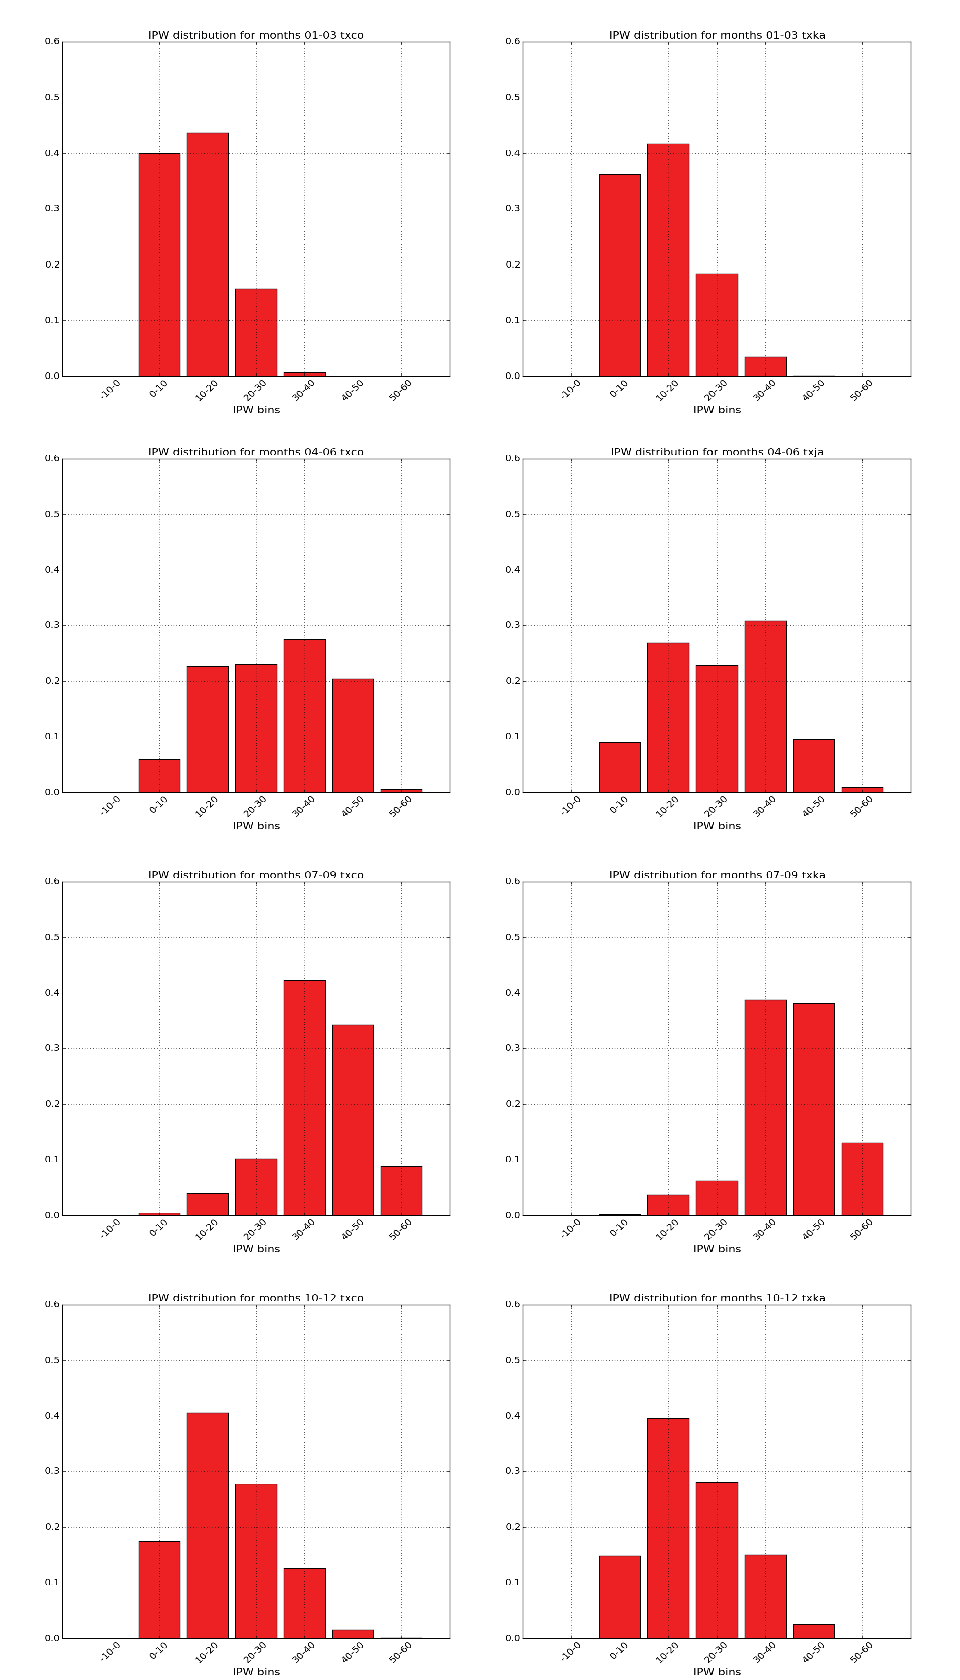
\includegraphics[width = 15cm,height = 20cm]{ipw_seasonal_distributions}
\caption{IPW distribution for 3 month periods for stations txco and txka}
\label{fig:ipw_seasonal}
\end{center}
\end{figure}
\subsection{IPW and Reflectivity Field Generation}
As a first step in the processes of correlating IPW and reflectivity fields and using spatial and temporal evolutions of both fields as predictor for severe weather in the near future(nowcasting), they were plotted on the same graph for visual inspections. Thus the reflectivity fields which were obtained for the KFWS radar from the NCDC data base(https://www.ncdc.noaa.gov/data-access/radar-data) and IPW values had to be converted to a common cartesian plot with respect to a fixed object(KFWS) radar in this case. 
\subsubsection{Radar Reflectivity Fields}
The radar reflectivity products used for this experiment are the level 3 radar base products measured at a $0.5^{\circ}$ elevation scan. The reflectivity are thus measured in $dBZ$ and are in polar coordinated. The radar reflectivity's obtained are in a $360 \times 230$ matrix where 230 is the number of range gates and 360 refers to a single sweep. The KFWS coordinates of the radar were placed from its lat long position to the center $(0,0)$ of the cartesian plot. The reflectivity is converted from the polar coordinates to the cartesian coordinates using the William's activation formula \cite{williams2014aviation}. The resolution of the cartesian plot was chosen to be 3km and $300 \times 300$ grid centered around the KFWS radar. Note that the range of the KFWS radar is circle of radius 230km, we use a smaller square domain of size $300 \times 300 \ km^2$ to be within the convex hull of the IPW stations.
\subsubsection{IPW fields}
Each GPS station were placed on the cartesian plot with respect to the KFWS radar converted from its latitude,longngitude location to the cartesian coordinates with respect to KFWS and the distances was measured using the formula given in \cite{williams2014aviation}. Each point measurement of NIPW were interpolated onto this domain of $300 \times 300 \ km^2$ centered around KFWS with a resolution of 3km. The technique that is used for interpolation is the Multiquadric interpolation approach given in \cite{tabios1985comparative}. Multiquadric interpolation is a weighted linear interpolation technique where the estimate $h_0$ for any grid point $(x_0,y_0)$ is given by 
\begin{equation}
h_0 = \sum_{j=1}^{n} w_j \cdot h_j
\end{equation}
where $w_j$ is the is the weight and $h_j$ is the observed NIPW at point $(x_j,y_j)$. In the Multiquadric technique the weights $w_j$ are calculated as the product of inverse of matrix of distances between observed points $(x_j,y_j)$ and distance between interpolated point and each observed point. This can be expressed as for each point $(x_j,y_j)$, 
\begin{equation}
h_j = \sum_{i=1}^{n} c_i \cdot d_{ji} \ \forall j = 1,2..n
\end{equation}
The coefficients $c_i$ are determined by 
\begin{equation}
c_i = \sum_{j=1}^{n} \delta_{ij} \cdot h_j \ \forall i = 1..n
\end{equation}
where $\delta_{ij}$ is an element of the inverse of the $n \times n$ distance matrix with elements 
$d_{ij}, j = 1..n \ and \ i = 1..n$ is the distance between the $ith$ and $jth$ observed points. 
Hence the interpolated point is given by
\begin{equation}
h_0 = \sum_{j=1}^n [\sum_{i=1}^n \delta_{ij} \cdot d_{0i}] \cdot h_j
\end{equation}
The weight can be expressed as 
\begin{equation}
w_j = \sum_{i=1}^n \delta_{ij} \cdot d_{0i}
\end{equation}
Expressing this in matrix notation if $D$ is the matrix $n \times n$ matrix of distances between each observed point, $U$ is a matrix of distances between $n \times k$ where $k$ is the number of interpolated points and $H$ is a vector of observed NIPW points. Then the NIPW field is given by $I$
\begin{equation}
I = [D^{-1} U]^{T} H
\end{equation}
The multiquadric technique can be summarized using the following algorithm
\begin{enumerate}
\item Map the locations of the n GPS stations from their latitude, longitude coordinates to x,y locations relative to some origin (e.g., relative to the location of the KFWS radar). The equations for calculating distances between latitude, longitude locations can be found in \cite{williams2014aviation}.
\item Define the n by n matrix of inter-site distances with entries $d_{ij}$.
\item Invert the distance matrix to obtain the n by n matrix of $delta_{ij}$.
\item Define the m by m Cartesian grid onto which the measurements are to be interpolated.
\item Construct the m by m by n matrix of interpolation weights.
\item Use equation (4.9) to obtain the interpolated field from the interpolation weights and the estimated NIPW values.
\end{enumerate}
%An algorithm for multquadric interpolation would thus proceed as follows:
%
%1.	Map the locations of the n GPS stations from their lat, lon coordinates to x,y locations relative to some origin (e.g., relative to the location of the KFWS radar). The equations for calculating distances between lat, lon locations can be found on the website (Williams aviation formulary).
%2.	 Define the n by n matrix of inter-site distances with entries dij.
%3.	Invert the distance matrix to obtain the n by n matrix of deltaij?s.
%4.	Define the m by m Cartesian grid onto which the measurements are to be interpolated.
%5.	Construct the m by m by n matrix of interpolation weights.
%6.	Use equation (4.5) to obtain the interpolated field from the interpolation weights and the estimated NIPW values.
\subsubsection{Radar IPW fields}
Once radar reflectivities and interpolated IPW fields were brought to the same coordinated, plots were made as shown in Figure \ref{fig:ipw_radar}. The fields were made at 30 minute intervals which is the sampling rate for IPW. The reflectivity fields had to be down-sampled to match the 30 minute rate. At a high level the goal of this Thesis is to exploit the spatiotemporal correlation between IPW an reflectivity fields to make predictions of precipitation 1 hour in advance. The radar and IPW field frames are the input to our machine learning algorithm which will be explained in the next section. 
\begin{figure}
\begin{center}
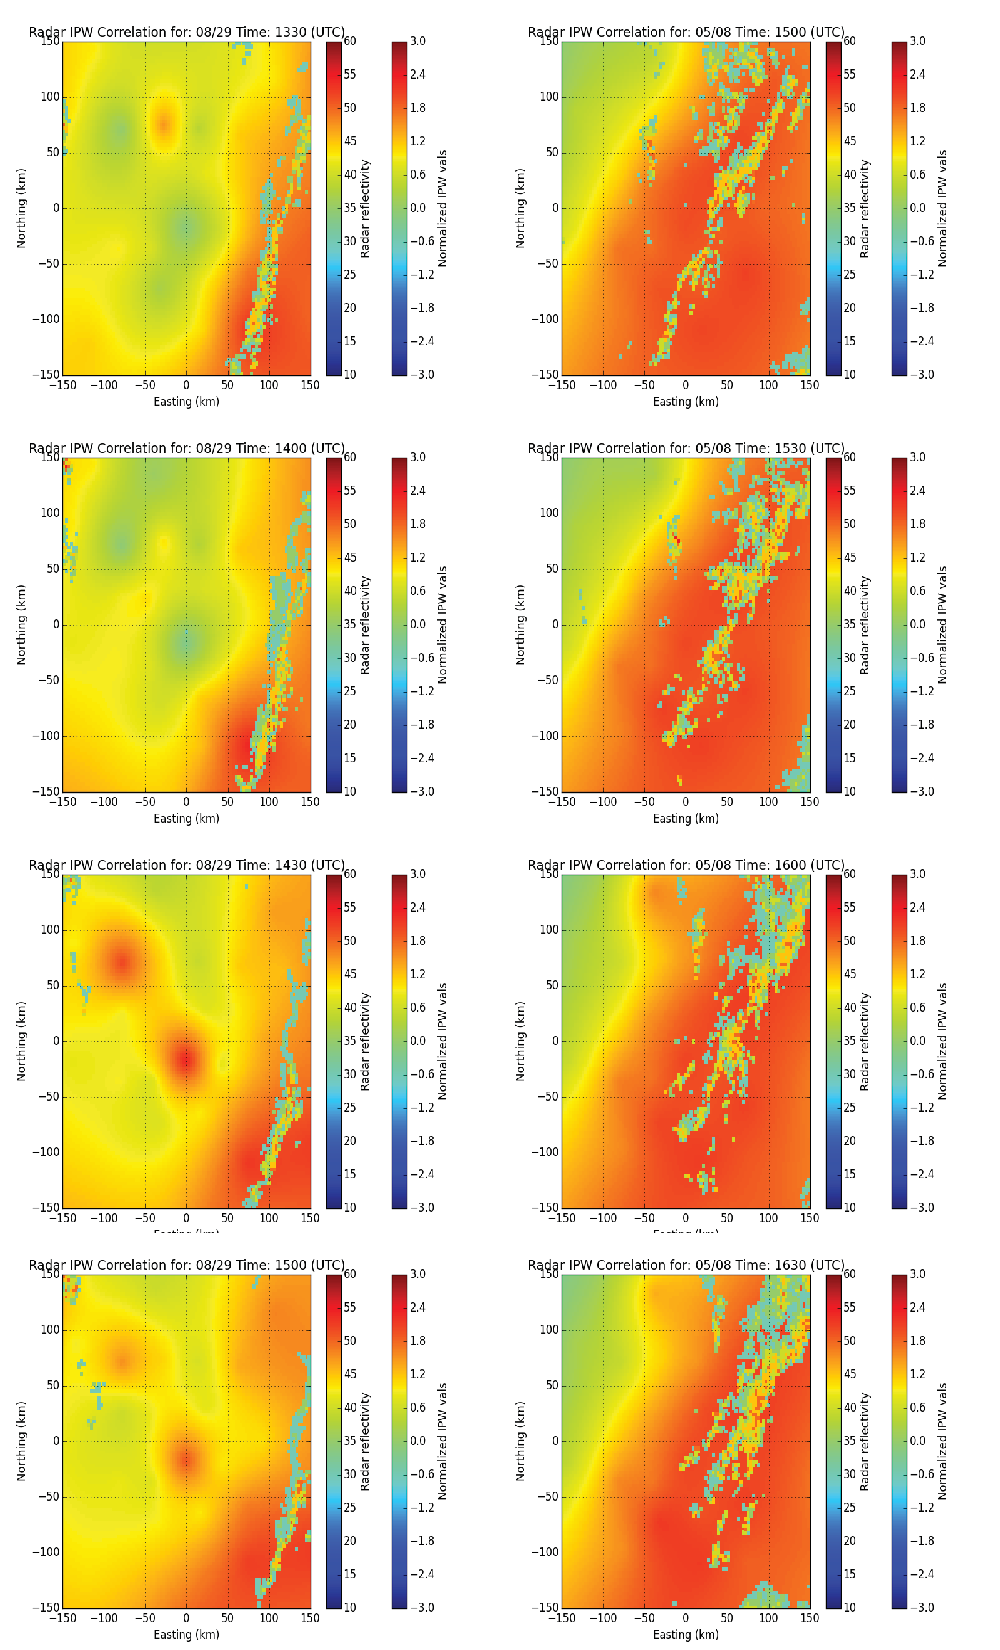
\includegraphics[width = 15cm,height = 20cm]{radar_ipw_fields}
\caption{Reflectivity fields overlayd onto IPW fields for two storms during August 29 and May 8th 2014}\label{fig:ipw_radar}
\end{center}
\end{figure}
\section{Determining training set}
A subset of days in the year of 2014 were chosen to do our experiments on. The days that we have chosen are from the months of May,July and August as it is during this time that heavy rainfall and convective storms are most likely to occur and these were the months where the noise in computed IPW values were the least. We define a "weather anomaly" as a day where if 30 or more IPW values from all stations evaluated on that day exceeded 2 standard deviations from the mean. Table \ref{table:weather anomaly} summarizes the 23 days chosen to do experiments on. 
\begin{center}
\begin{tabular}{ |c|c|c| } 
 \hline
 May & July & August  \\ 
 \hline
 08 & 15 & 11 \\ 
 09 & 16 & 16 \\
 12 & 17 & 17 \\
 13 & 18 & 18 \\
 23 & 28 & 19 \\
 24 & 29 & 29 \\
 25 & 30 &      \\
 26 & 31 &      \\
 31 &     &       \\
\hline
%\caption{Days chosen to perform nowcasting experiments on. All times chosen are UTC time}\label{table:weather anomaly}
\end{tabular}
\end{center}


\section{Nowcasting Algorithm}
The nowcasting algorithm that will be developed in this Thesis will determine the state of the atmosphere in the next hour, based on the current and past patterns of the reflectivity and IPW fields.An initial approach to the problem is to predict the state of each of the 10,000 pixels in our domain. Each pixel is defined as a random variable $Y \in \ {(0,1)}$, where 0 is defined as "no rain" for that hour and 1 is defined as "rain" for that hour, and the rain is defined as the case where the reflectivity the reflectivity value at that pixel exceeds 24dBz. 

The feature set for determining the dependent variable $y$ is chosen to be as 4 frames of IPW fields and 4 frames of reflectivity fields. Since each frame of reflectivity or IPW field contains 10,000 pixels, it is not feasible to include all 10,000 pixels of IPW and reflectivity field to predict the state of each pixel in the next hour. Initially we choose an arbitrary set of pixels consisting of a $33 \times 33$ grid around the pixel that is considered for prediction. The arbitrary IPW and reflectivity field are shown in Figure \ref{fig:example_33_cross_33} and 4 frames if IPW and reflectivity fields were chosen to predict the state of a pixel. We define two random variables $I^t \in \mathbb{R}^D$ for the IPW field at time step t and $R^t \in \mathbb{R}^D$ for the reflectivity at time step t where $D = 1089 (33 \ \times \ 33)$ and t is the time in hours. 

\begin{figure}
\begin{center}
\includegraphics[width = 10cm,height = 10cm]{example_fields}
\caption{Example of arbitrarily  chosen 33 x 33 IPW and reflectivity field around the pixel for which prediction is being made}\label{fig:example_33_cross_33}
\end{center}
\end{figure}

The learning problem is defined as set of examples pairs $T$ = $\left\{(\textbf{$x_i$},y_i^{t^*}), i = 1:N\right\}$ where \textbf{$x_i$} = $(I_i^{t^*-2.5},I_i^{t^*-2},I_i^{t^*-1.5},I_i^{t^*-1},R_i^{t^*-2.5},R_i^{t^*-2},R_i^{t^*-1.5},R_i^{t^*-1})$
%$T$ = $\left\{(I_i^{t^*-2.5},I_i^{t^*-2},I_i^{t^*-1.5},I_i^{t^*-1},R_i^{t^*-2.5},R_i^{t^*-2},R_i^{t^*-1.5},R_i^{t^*-1},y_i^{t^*}), i = 1:N\right\}$ 
, N is the number of training examples, we try and learn a function such that $f:\mathbb{R}^D \  \to Y $.
\subsection{Initial Classifications}
As an initial step we simplify the problem at hand to evaluate the viability of our approach and to evaluate simple classifiers on the data set. We make the following two simplifications to the problem. 
\begin{enumerate}
 \item We reduce the domain from the larger $300 \ \times \ 300 km^2$ grid to a smaller $ 33 \ \times \ 33 km^2$ grid consisting of 1089 points in the days of our interest. 
  \item The IPW and reflectivity field at each time step is averaged, which significantly reduces our feature space from the initial $ D = 8712$ ($1089 \ \times \ 8$) to $D = 8$. 
\end{enumerate}
A summary of the experimental data set $T$ is given in Table. The total number of examples was obtained by $1089 \times 23 \times 48 = 1,202,256$ where we have 1089 pixel points in our domain from 23 days and each day has 48 observations (observations made at 30 minute sampling rate). The number in the Table \ref{table:data_statistics} is slightly lesser than 1,202,256 because for the starting of in new UTC day we do not have the 4 hours prior IPW and reflectivity fields. We can also see that the total number of rain cases is only 5 \% of the entire experimental data set. 


\begin{table}
\begin{center}
\begin{tabular}{|c|c|c|}
\hline
Number of examples & Number of no rain cases & Number of rain cases \\
\hline
\hline
1,153,251  & 1,104,819 & 48,432 \\
\hline
\end{tabular}
\caption{Data statistics}
\label{table:data_statistics}
\end{center}
\end{table}

The experimental set was broken down into a series of training set and validation sets. This was done using the K-fold cross validation technique \cite{friedman2001elements} where $k=7$. The algorithm for the cross valiation technique is explained as follows. 

\begin{enumerate}
\item Randomly shuffle the experimental data set. 
\item Divide the experimental data set into K equal parts.
\item Train on K-1 blocks and test on the $(K-1)^{th}$ block. 
\item Repeat until all K blocks have been tested on using the other K-1 blocks as training examples. 
\end{enumerate}

Two simple classifiers were trained and tested using this method The Naive Bayes Classifier and the Random Forest Classifier. 

\subsection{The Naive Bayes Classifier }

The Na�ve Bayes or the Bayes optimal classifier \cite{zhang2004optimality} is based on the simple assumption that each variable behaves independently with respect to the other variables and disregards any correlation one variable may have on any other. Given a training example $x_i \in \mathbb{R}^D$ and its corresponding output $Y_i = c$ where $c \in G$ and G is a set of all possible classes we can compute the prior probability $P(Y = c) = \pi_c$ and the true probability $\phi_c(x) = p(X = x | Y = c)$.  If we apply the Bayes rule to calculate the posterior probabilities
\begin{equation}
P(Y = c | X = x) = \dfrac{\phi_c(x) \pi_c}{\sum_{c' \in Y}\phi_{c'}(x) \pi_{c'}}
\end{equation}
Making the "Naive" assumption that all variables are independent we can say that
\begin{equation}
\phi_c(x) = p(X = x | Y = c) = \prod_{d=1}^{D} p(X_d = x_d | Y = c) = \prod_{d=1}^{D}\phi_{cd}(x_d)
\end{equation}
Thus we can write the general classification function as 
\begin{equation}
f_{NB}(x) = \operatornamewithlimits{argmax}\limits_{c \in Y} \pi_c \prod_{d = 1}^{D} \phi_{cd}(x_d)
\end{equation}
The Naive Bayes classifier despite making a fundamental assumption of independent variables, which is never true in real world problems, is capable of forming complex decision boundaries.

\subsection{Random Forest Classifier}
The random forest classifier consists of an ensemble of CART(Classification and Regression Trees) where the decision on deciding the class variable is made on a collective vote of the individual decision trees in the forest \cite{breiman2001random}. The random forests builds a large collection of decorrelated trees and averages them. Trees are ideal candidates for random forests as they can capture complex interactions in the data. 

%The decision tree classifier is similar to a binary tree. Classification is based on a particular feature variable xd being greater than, less than or equal to a certain threshold t. where x is a vector of inputs with D features associated with it. The data case is assigned to the left or right of the tree based on the feature variable (xd ) and the threshold(t). The data cases are traversed through the tree from the root node to the leaf of the tree, where the class is determined at the leaf. The decision trees decide on the feature d and a threshold t based on a greedy heuristic which tries to maximize the training accuracy.
%
%In a geometrical sense the decision tree tries to break the D dimensional feature space into smaller regions. The goal of the decision tree is to hence break up these regions such that a region has maximum number of points or inputs that belong to the same class. Hence a fundamental metric pkm is the proportion of observations in the mth region that are in the kth class. Generally the pkm is minimized for finding the decision tree parameters d and t

A simple decision tree works on the principle of finding a best split amongst all variables $d \in D$ given a set of training vectors and output pairs $(x,y)$ where x is a vector with dimension D. Classification is based on finding a threshold $t$ such that a variable in a data case $x_d$ is split based in $x_d < t \ or \ x_d > t or \ x_d =t$. The data case is assigned to the left or right of the tree based on $x_d$ and threshold t. The data cases are traversed through the tree from the root node to the leaf of the tree, where the class is determined at the leaf.

The learning of the decision tree works by finding the optimal variable $d$ to split on and the threshold $t$ using a greedy heuristic that tries to maximize on training accuracy. In a geometrical sense the decision tree tries to break the D dimensional feature space into smaller regions. The goal of the decision tree is to hence break up these regions such that a region has maximum number of data cases that belong to the same class. Hence a fundamental metric $p_{km}$ is the proportion of observations in the mth region that are in the kth class. Generally the $p_{km}$ is minimized for by finding the decision tree parameters d and t. The "Genie Index" criterion is used to maxamize the training accuracy given by

%The learning of a decision tree works using a greedy algorithm where thrasholds are found to split at each node that tries to maxamize a certain criteria which in our case is maxamizing classification accuracy. This criteria is usually the which is defined as 
\begin{equation}
C_{GI} =  \sum_{k=1}^{K} p_{km} (1 - p_{km})
\end{equation}
 The decision tree construction proceeds recursively to find the optimal variable and threshold pair according to a given criteria and a specific depth of the tree. 
 
 The random forest algorithm thus can be summarized by the following algorithm from \cite{friedman2001elements}. 
 
\begin{enumerate}
\item Initialize the number of trees B in the forest. 
\item for b = 1:B
\begin{enumerate}
\item Draw a bootstrap sample Z of size N examples from the training data
\item Grow a random forest tree $T_b$ to the bootstraped data by recursively repeating the following steps
\begin{enumerate}
\item select m at random from D (ideally $m = \sqrt{|D|}$)
\item pick the best variable split among the m variables based on the Genie criteria
\item split the node to two daughter nodes
\end{enumerate}
\item The classification is based on the majority votes from B trees. 
\end{enumerate}
\end{enumerate}

The random forest thus forms its "decorrelated" trees by picking a set of random variables m at each iteration of each tree. In this fashion an ensemble of weak learners are built.

 One of the key advantages of the Random Forest classifier is its interpretability through variable importance. The variable importance is an attribute of random forest classifier which measures the relative importance of each variable. This is done by measuring the prediction performance of the "OOB(Out Of Box Samples)". When the $b^{th}$ tree is being constructed in the forest, examples apart from its bootstrapped samples are used to measure the predictive performance at a particular split. Different permutations of the variable split are tried and the performance are measured using the OOB. This accumulates over all the trees and the variables which are most important are ranked.
 
 \section{Evaluating the Performance of the Nowcasting Algorithm}
 
To evaluate the performance of the Nowcasting we chose a set of metrics to measure its performance which are tailored for this problem where we only have $~5 \%$ of the experimental set with rain cases. So a measure on how well we predict rain is needed. First a measure of a simple true positive rate, true negative rate, false positive rate and false negative rate are measured and enumerated in contingency table. 

We then define precision(P) and recall(R) as follows \cite{powers2011evaluation} 
\begin{figure}[!t]
\begin{center}
\includegraphics[width = 15cm,height = 10cm]{initial_results}
\caption{Average precision score for (a) Gaussian Naive Bayes Classifier (b) Random Forest Classifier}\label{fig:initial_results}
\end{center}
\end{figure}

\begin{equation}
P = \dfrac{T_p}{T_p + F_p}
\end{equation}
\begin{equation}
R = \dfrac{T_p}{T_p + F_n}
\end{equation}
Precision is the measure of confidence or the proportion of cases that are predicted positive are actually positive. Recall is a measure of sensitivity or the proportion of real positive cases that are predicted positive. A system with high recall but low precision may indicate that that the predictor is returning a lot of cases of rain but only few are actually correct. A system with low recall but high precision indicates that the predictor is returning very few positive results but most of these results are accurate. Ideally a good balance between the two scores is desirable and thus we define the statistical $F_1$ score as
\begin{equation}
f_1 = 2 \cdot \dfrac{P \cdot R}{P + R}
\end{equation}
\begin{figure}[!t]
\begin{center}
\includegraphics[width = 15cm,height = 12cm]{random_forest_feature_importance}
\caption{Relative variable importance measured by random forest classifier}\label{fig:variable_importance}
\end{center}
\end{figure}
\section{Nowcasting Results}
With our initial data set prepared and two simple but diverse classifiers chosen along with a sound evaluation metric, we can now make predictions to evaluate the viability of the nowcasting algorithm. 


Three kinds of predictions were made using the two classifiers on each of the 7 training and validation sets described above.
\begin{enumerate}
\item Predicting with only past IPW fields
\item Predicting with only past Reflectivity fields
\item Predicting with IPW and Reflectivity fields
\end{enumerate}

Figure \ref{fig:initial_results} shows the average precision curve for the two classifiers using a combination of the three variables. The curve was drawn by varying the threshold probability and plotting the corresponding value for precision and recall. The average precision score is then determined by the area under the precision curve.  It can be seen in both classifiers that using using IPW alone or using Reflectivity alone does not perform as well as using both IPW and Reflectivity. In the random forest classifier there is a significant increase in average precision score from using reflectivity only to predict to using both IPW and reflectivity to predict. The increase is from 0.53 to 0.73 average precision score. 

The Naive Byes classifier does not seem to perform well at all. This is because of the assumption that all of the variables are assumed to be independent of each other. In this case there is a correlation between the $t-1.5$ and the $t-1$ variable for both IPW and reflectivity fields. This is one of the main reasons that this classifier does not perform as well as the random forest classifier.

\begin{figure}[!t]
\begin{center}
\includegraphics[width = 15cm,height = 10cm]{f1_scores}
\caption{$f_1$ score for each train validation set}\label{fig:f1_scores}
\end{center}
\end{figure}

The Random Forest Classifier seems to show promising results with an average precision score of 0.73. Figure \ref{fig:variable_importance} shows the relative variable importance for the classification done given the input of IPW and reflectivity fields. The top 4 most important variables used by the random forest to make its prediction are the IPW and reflectivity fields measured at the $(t-1)^{th}$ time step and the $(t-2.5)^{th}$ time step.

Figure \ref{f1_scores} plots the $f_1$ score for both classifiers using each of each of the variable sets for each train validation set. The random forest classifier has an average $f_1$ score of 0.68 and does not vary much from validation set to validation set. This implies that that all all of the misclassified examples are of a very specific type and they are also equally distributed between the validation sets. 



\chapter{Contributions, Plans and Expected Timeline}

To gain competency in the area of GPS-Metrology and knowledge about its workings to conduce research, GPS Met sensors were developed and deployed in the field to produce near real time water vapor estimates. The following section describes development of a GPS-Met sensor. 

\section{GPS-Metrology Sensor Development}

A major goal achieved by this project is the development of low cost GPS-Met sensors to be used in dense network of GPS-Met stations for better spatial and temporal sampling of water vapor. Two such systems were developed 'CNVL' and 'NWSD' and deployed at the University of Texas Arlington and the National Weather Services Weather Forecast office in Dallas Fort-Worth area as shown in Figure \ref{fig:GPS_Met_Stations}. The system consists of a dual frequency GPS receiver, a high precision barometer and vaisala WXT-510 weather station. The cost of building each of these GPS-Met stations was around \$5,000. This is significantly lower than any other GPS station which is currently operated by NOAA, SuomiNet or SOPAC. Both CNVL and NWSD were validated with near real-time IPW values published by nearby stations operated by NOAA. 

Software was developed and installed on a laptop running windows OS at the node which periodically retrieved data from each of the sensors and placed them in files with the correct naming conventions as defined by IGS\cite{moore2004igs}. Both stations also meet the many requirements of the IGS site guidelines \cite{moore2004igs} for classification as a continouseley operated GPS station. 

Software was developed to download the data periodically through FTP to a server at UMASS(emmy9) which processed the RINEX files to produce near real-time precipitable water vapor products published online every hour(http://emmy9.casa.umass.edu/gpsmet/). The processing for near realtime precipitable water is done through the GAMIT software \cite{herring2015gamit} and scripts were developed to automate the processes periodically. Currently development is under way for a front end which makes it easier for the user to locate each of the site on a map and view the real-time water vapor products. Development of a third station is also under way which is to be deployed at UMASS by the end of the year. For further details about the project refer (cite AMS 2015 here). 

\section{Tentative Plan}

We propose to make better precipitation predictions using the feature fusion method of CCA as described above and evaluating the predictive potential of this new feature space with an artificial neural network, which has shown promising results in many other fields. This would then motivate other work to try and use the CCA using other spatial fields and see the results on predictions. The next step would naturally be to predict the amount of precipitation rather than just as a binary output. 

We propose two methods for the prediction the amount of precipitation 1 hour in advance as follows. 
\begin{enumerate}
\item Treat this as a regression problem and predict the output reflectivity field similar to \cite{french1992rainfall}. 
\item Treat this as a multi class classification problem and discretize the different reflectivity values into equally sized bins. 
\end{enumerate}

\section{Expected Contributions}

The expected contributions of this theses are as follows. 

\begin{enumerate}
\item Building spatial fields of IPW derived from a dense network of GPS-stations using the multiquadric technique
\item Using a machine learning approach for nowcasting using the GPS derived IPW products for nowcasting. 
\end{enumerate}


\begin{figure}[!h]
\begin{center}
\includegraphics[width = 15cm,height = 10cm]{GPS_Met_Stations}
\caption{GPS Met station (a), (c) CNVL at University of Texas Arlington and (b), (d) NWSD at Weather Forecast Office DFW}\label{fig:GPS_Met_Stations}
\end{center}
\end{figure}

\appendix
\chapter{Meta Data}

\chapter{THE SECOND APPENDIX TITLE}
...

\backmatter  %% <--- mandatory


\interlinepenalty=10000  % prevent split bibliography entries
\bibliographystyle{umassthesis}
\bibliography{umthsmpl}
\end{document}

%%% Local Variables: 
%%% mode: latex
%%% TeX-master: t
%%% End: 
